\documentclass{standalone}
\usepackage{tikz}

\begin{document}
    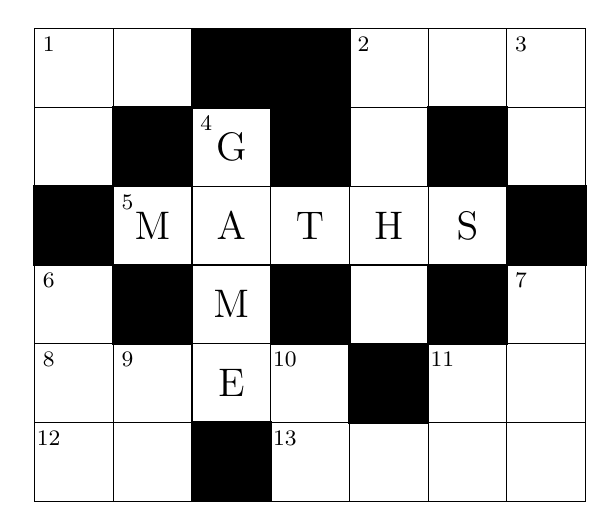
\begin{tikzpicture}
        \begin{scope}[shift={(-1.5,-1.5)}]
            \draw (0,0) grid (7,6);
        \end{scope}
        \node at (0,2) {\Large M};
        \node at (1,2) {\Large A};
        \node at (2,2) {\Large T};
        \node at (3,2) {\Large H};
        \node at (4,2) {\Large S};
        \node at (1,3) {\Large G};
        \node at (1,1) {\Large M};
        \node at (1,0) {\Large E};
        
        \foreach \i/\j in {0/1,-1/2,0/3,1/4,2/3,2/4,2/1,1/-1,4/3,5/2,3/0,4/1}{
            \node[draw,thick,fill=black,minimum size=1cm] at (\i,\j) {};
        }
        
        \begin{scope}[shift={(-0.32,0.3)}]
            \node at (-1,4) {\footnotesize 1};
            \node at (3,4) {\footnotesize 2};
            \node at (5,4) {\footnotesize 3};
            \node at (1,3) {\footnotesize 4};
            \node at (0,2) {\footnotesize 5};
            \node at (-1,1) {\footnotesize 6};
            \node at (5,1) {\footnotesize 7};
            \node at (-1,0) {\footnotesize 8};
            \node at (0,0) {\footnotesize 9};
            \node at (2,0) {\footnotesize 10};
            \node at (4,0) {\footnotesize 11};
            \node at (-1,-1) {\footnotesize 12};
            \node at (2,-1) {\footnotesize 13};
            
        \end{scope}
    \end{tikzpicture}
\end{document}